\documentclass[../main.tex]{subfiles}
\begin{document}
\section{Introduction}

Since the mid-1980s, real interest rates in many advanced economies, including Denmark, have followed a protracted downward trend and slumped to remarkably low levels in recent years, see Figure \ref{fig:demographics_real_interest_rateDK}\textcolor{blue}{A}. This development has recently been associated with a decline in the natural rate of interest (NRI). The NRI characterises the real interest rate in an economy that follows its long-term trend with the output gap closed (\textcite{wicksell1936interest}).\footnote{In other literature, the NRI is also defined as the equilibrium real interest rate, natural real rate or $r^*$.} In general, there are two main determinants proposed to explain the decline in the NRI, namely productivity slowdown and shifts in saving behaviour due to demographic changes. This paper mainly focuses on the impact of demographics from a modelling perspective. Like most other developed countries, Denmark is undergoing a significant demographic transition where higher life expectancy and low fertility lead to an ageing population. As illustrated in Figure \ref{fig:demographics_real_interest_rateDK}\textcolor{blue}{B}, the Danish old-age dependency ratio, defined as the ratio of people aged 65 and above relative to people aged 20-64, is projected to increase from around 20 percent in the 1960s to over 45 percent in 2040 and beyond. This will put downward pressure on the NRI as private savings increase to finance consumption in retirement, which depresses the marginal product on capital and thus the NRI.

By applying an open economy OLG framework on Denmark with detailed demographic data and taking a realistic representation of the public pension system into account, we find that the Danish NRI has declined by 1.8 percentage points between 1985 and 2020. Demographics account for approximately half of this decline.  Decreasing mortality risk (higher life expectancy) accounts for 0.7 percentage points and low fertility by another 0.2 percentage points. The rest of the decline is mainly due to sluggish global total factor productivity (TFP) growth. Additionally, demographic factors are projected to put further downward pressure on the real interest rate in the near future. 

\begin{figure}[H]
\caption{Long run tendencies for the Danish economy}
\label{fig:demographics_real_interest_rateDK}
        \centering
        \begin{minipage}{0.45\textwidth}
            \centering
            \subcaption{\footnotesize \textbf{A. Real interest rate (\%)}}
            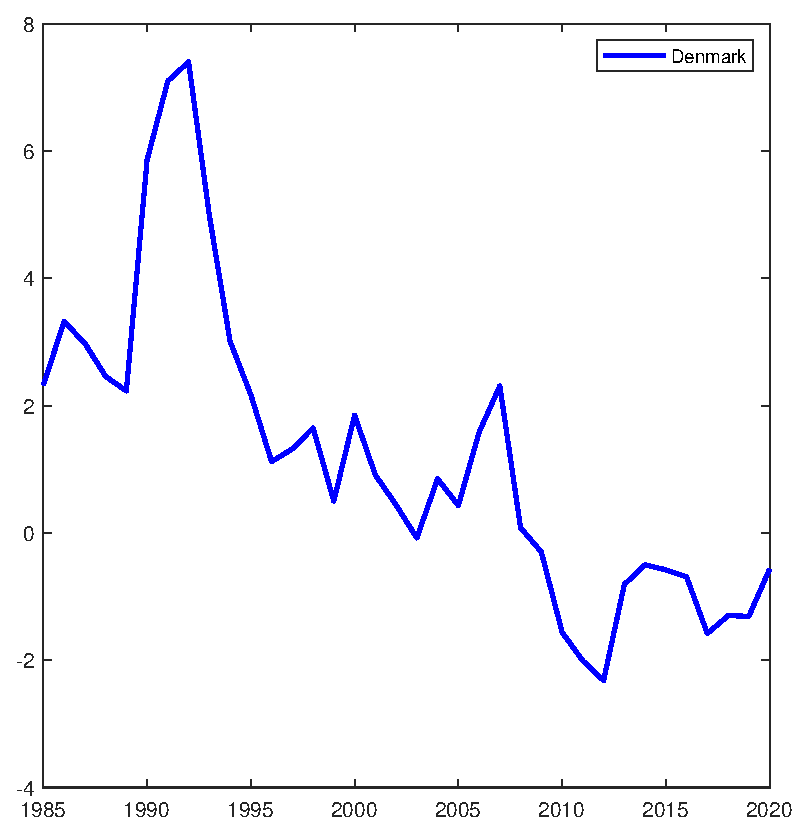
\includegraphics[width=0.95\textwidth]{Figures/Figure_0.eps} % first figure itself
        \end{minipage}
        \begin{minipage}{0.45\textwidth}
            \centering
            \subcaption{\footnotesize \textbf{B. Old-age dependency ratio (\%)}}
            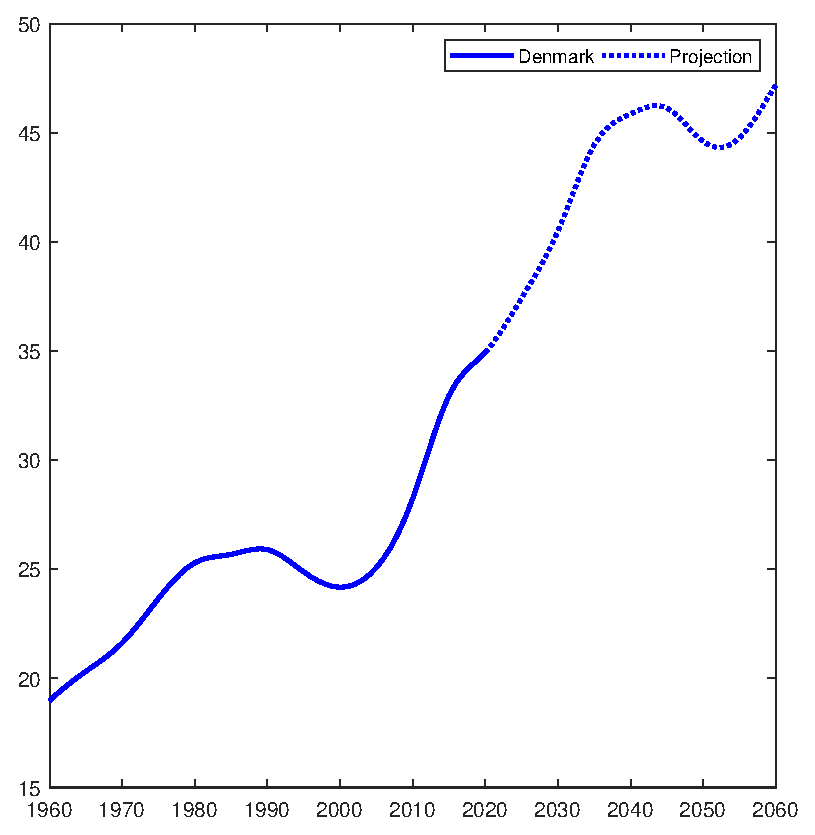
\includegraphics[width=0.95\textwidth]{Figures/Figure_1B.eps} % second figure itself
        \end{minipage}
        \begin{fignote}
                \textit{Note:} Data for the real interest rate is Nationalbanken's \textit{diskonto} minus inflation (consumer price index), table DNRENTA and PRIS9 from Statistikbanken, respectively. Demographic data is from UN World Population Prospects 2019 (medium-fertility variant). The old-age dependency ratio is defined as the ratio between the number of people aged 65 and above relative to the number of people aged 20-64.
                \end{fignote}
    \end{figure}

Furthermore, we explore what ageing implies for the public pension system and monetary policy. In low interest rate environments, there are limited possibilities for conventional monetary policy as an instrument to stimulate economic activity and generate growth, making it difficult to break out of secular stagnation defined as a period with low growth and low interest rates (\textcite{summers2014us}). In response to the demographic transition, the Danish government has proposed to reform the public pension system. We incorporate actual proposals to increase the retirement age and decrease pension benefits into the model. We find that lower pension benefits will put further downward pressure on the NRI as workers increase their savings to finance consumption during retirement. On the contrary, a higher retirement age contributes to an increase in the NRI because workers save less in anticipation of a shorter retirement period.  

Several international studies have investigated how the demographic transition has affected the NRI in developed economies. We use the model setup by \textcite{bielecki2020demographics} which allows us to incorporate detailed Danish registry data combined with demographic data from the UN. Unlike \textcite{gagnon2021understanding} and \textcite{carvalho2016demographics} who use tractable life-cycle models of a closed economy to estimate the NRI in the US and a representative developed economy, respectively, we model a small open economy to incorporate the effect of cross-border capital flows in our analysis of the development in the NRI. \textcite{gagnon2021understanding} find that the demographic transition is almost the sole culprit of the decline in the NRI in the US by 1.25 percentage points since 1980. \textcite{carvalho2016demographics} find that demographics account for about half of the total decline in the NRI by 1.5 percentage points between 1990 and 2014 in a representative developed economy. \textcite{eggertsson2019model} also apply a quantitative life-cycle model and find that demographic changes are the main forces behind secular stagnation in the US. From a Danish perspective \textcite{pedersen2015danish} finds that the NRI in Denmark was close to 0 around 2015, possibly negative, and has been on a long-term negative trend.  

The results in this paper are generally in line with these recent findings suggesting that the demographic transition is an important factor for the decline in the NRI. The paper is structured as follows. Section \ref{sec:The_model} describes the model setup used in this paper. We present our calibrations based on data in Section \ref{sec:calibrations}. The main results, including a decomposition of the NRI, are presented in Section \ref{sec:results}. We analyze the policy implications, namely pension system reforms and monetary policy instruments, in Section \ref{sec:policy_implications}. In Section \ref{sec:Discussion}, we discuss the model selection as we consider limitations within the setup and a possible extension to the model. In Section \ref{sec:conclusion} we summarize and conclude.
\end{document}